% Preamble
%\documentclass[xetex,mathserif,serif]{beamer}
\documentclass{beamer}

% Packages
\usepackage[spanish]{babel}
\selectlanguage{spanish}
\usepackage[utf8]{inputenc} % For spanish (and international) letters like acents.
\usepackage{hyperref} % To create hyperlinks within the document.
\usepackage{graphicx} % To include graphics (pictures, images)
\usepackage{float} % For the use of the parameter "H" in command "\begin{figure}[H]" (i.e. exact position of image in text)
\usepackage{verbatim} % For long comments
\usepackage{tikz} % For include Dia diagrams in .tex format

\graphicspath{{../Diagramas/}} % Path of the folder containing the images

\title{Colección Archivística del LAIS}
\subtitle{Sistema de apoyo a la catalogación de archivos audiovisuales}
\author{Rodrigo Colín Rivera}
\institute
{
  Laboratorio Audiovisual de Investigación Social\\
  Instituto de Investigaciones Dr. José María Luis Mora
}
\date{\today}
\subject{Catalogación de Acervo Documental en Video}

\begin{comment}
\AtBeginSection[]
{
  \begin{frame}
    \frametitle{Tabla de contenidos}
    \tableofcontents[currentsection]
  \end{frame}
}
\AtBeginSubsection[]
{
  \begin{frame}
    \frametitle{Tabla de contenidos}
    \tableofcontents[currentsection,currentsubsection]
  \end{frame}
}
\end{comment}

% Style and theme
%\usetheme{Warsaw}
\usecolortheme{orchid} %crane,dolphin,lily

% Document environment
\begin{document}

\frame{\titlepage} % Página inicial

\section{Antecedentes y problemática actual}
\begin{frame}
	\frametitle{Introducción}
	El resguardo y documentación de materiales audiovisuales constituye una tarea prioritaria entre quienes recurrimos a ellos cotidianamente con fines de investigación. El Laboratorio Audiovisual de Investigación Social (LAIS) del Instituto de Investigación Dr. José María Luis Mora se propusó abocarse a esta labor para construir un acervo debidamente documentado, ponerlo en acceso para consulta y potenciar así la investigación con este tipo de materiales.
\end{frame}

\begin{frame}
	\frametitle{Antecedentes y problemática actual}
	El LAIS consta de una colección archivística para materiales audiovisuales cuyos registros actuales se encuentran en formato de \textbf{hojas de cálculo} (mediante Excel) que integran la ficha de documentación de cada material audiovisual.
	
	La problemática principal con esta manera de catalogación es que resulta \textbf{complicado buscar} o filtrar los registros. Además de otros problemas como La integridad de la información, la cantidad de usuarios que pueden consultar estos registro, la manipulación de los datos y el acceso a esta información.
\end{frame}

\section{Propuesta para el sistema de apoyo a la catalogación de archivos audiovisuales}
\begin{frame}
	\frametitle{Propuesta}
	\framesubtitle{Creación de un sistema computacional}
	
	La propuesta consiste en crear una \textbf{base de datos} para el manejo actual y futuro de las fichas de documentación de los materiales audiovisuales del LAIS junto con una \textbf{interfaz} de usuario que permita manipular fácilmente la base de datos.
\end{frame}

\subsection{Comparación entre hojas de cálculo y base de datos}
\begin{frame}[shrink]
	\frametitle{Propuesta}
	\framesubtitle{Comparaciones entre hojas de cálculo y base de datos}
	
	\begin{center}
		\begin{tabular}{| l | p{6.5cm} | p{6.5cm} |}
			\hline
			 & Hoja de cálculo & Base de datos \\ \hline
			 
			 Objetivo 
			 	& Realizar cálculos numéricos a través del uso de diversas fórmulas aritméticas. 
			 	& Almacenar datos en un servidor. \\
			 \hline
			 Almacenamiento
			 	& En archivos (libros) que contienen una o varias hojas de cálculo con filas y columnas para describir los datos.
			 	& En tablas que contienen registros (renglones) donde cada valor le corresponde un tipo de dato (columna)\\
			 \hline
			 Manejo
			 	& Cualquier persona con un conocimiento básico puede manipular, ordenar o filtrar datos.
			 	& Programador o persona encargada de la base de datos realiza consultas a través del lenguaje de programación SQL (\textit{Structured Query Language}). Requiere una interfaz de usuario para una fácil manipulación de la base. \\
			 \hline
			 Complejidad (datos)
			 	& Los datos son sencillos de manejar pero a mayor cantidad, mayor complejidad.
			 	& El modelo relacional permite mantener unidades organizadas para los datos (tablas) \\
			 	\hline
			 Repetición de datos
			 	& Se pueden presentar repetición o redundancia de datos.
			 	& Si el diseño de la base de datos es correcta, no se permite redundancia de información. \\
			 	\hline
			 Modificaciones
			 	& Una sola persona puede modificar a la vez. Varias personas con copia del original pueden hacer modificaciones pero al combinar la información queda sujeta a errores humanos.
			 	& Los manejadores (programas) de bases de datos permite multiusuarios y mecanismos de control en las modificaciones. \\
			 	\hline
			 Presentación
			 	& Adecuado para incrustar en documentos escritos o mostrar gráficas relativas a los datos contenidos.
			 	& Solamente a través de una interfaz de usuario se pueden presentar los datos. El formato varia según la implementación. \\
			 	\hline
		\end{tabular}
	\end{center}
\end{frame}

\section{Esquema general del sistema}
\begin{frame}
	\frametitle{Esquema general del sistema}
	Para la manipulación de la base de datos (consultar, buscar, insertar y borrar registros) se debe crear una interfaz intuitiva para los usuarios.
	La siguiente figura muestra el diseño general separando la \textbf{base de datos} de la \textbf{aplicación web} y mostrando las responsabilidades o usos de cada tipo de usuario (programador, interno del LAIS y usuario externo al LAIS).
\end{frame}

\begin{frame}
	\begin{figure}[H]
		\centering
		\includegraphics[width=0.8\textwidth]{EsquemaGeneral.png}
		\caption{Esquema general del sistema de consulta}
		\label{fig:esquema_general}
	\end{figure}
\end{frame}

\subsection{Casos de uso}
\begin{frame}
	\frametitle{Casos de uso}
	Los casos de uso son un tipo de diagrama que permite representar a los usuarios involucrados y las principales acciones del sistema.
	Las acciones básicas son: \textbf{consultar}, \textbf{buscar}, \textbf{agregar} y \textbf{editar} un material audiovisual.
\end{frame}

\begin{frame}
	\begin{figure}[H]
		\centering
		\includegraphics[width=0.8\textwidth]{CasosDeUso.png}
		\caption{Diagrama de casos de uso}
		\label{fig:caso_de_uso}
	\end{figure}
\end{frame}

\section{Selección de tecnologías}
\begin{frame}
	La selección de tecnologías está orientada en utilizar herramientas y estándares ampliamente aceptados y probados:
	\begin{description}
		\item[MySQL] Sistema manejador de bases de datos.
		\item[MySQL Workbench] Herramienta de apoyo a la administración de la base de datos.
		\item[PHP] Lenguaje de programación orientado a servidores (para realizar conexiones a la base).
		\item[HTML5] Lenguaje para la creación de la interfaz web (páginas web).
		\item[Bootstrap] Biblioteca adicional para diseño web responsivo.
		\item[Javascript] Lenguaje de programación auxiliar para manejor de eventos.
		\item[jQuery] Biblioteca auxilar para manipulación de páginas web.
	\end{description}
\end{frame}

\section{Diseño de la base de datos}
\begin{frame}
	\frametitle{Diseño de la base de datos}
	Las \textbf{tablas} y los \textbf{campos} (\textbf{columnas}) que lo conforman están basadas en la descripción archivística existente en hojas de cálculo que hasta el momento han sido el modelo a seguir para la catalogación archivística.
\end{frame}

\begin{frame}
	\begin{figure}[H]
		\centering
		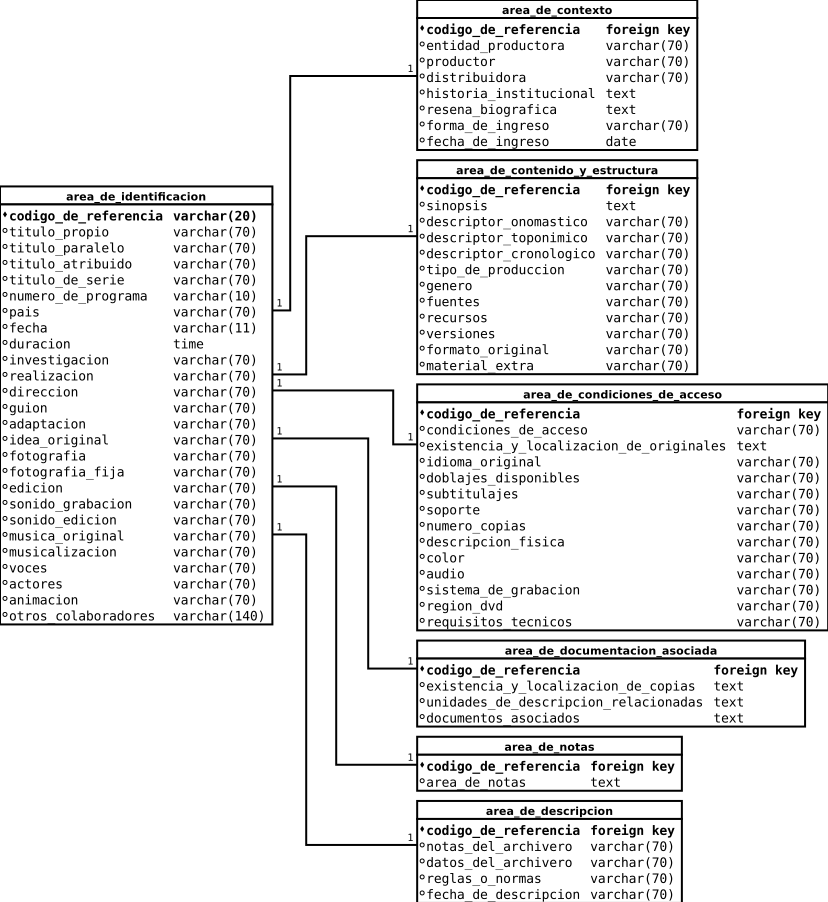
\includegraphics[keepaspectratio=true,scale=0.2]{EntidadRelacion.png}
		\caption{Diagrama Entidad-Relación que muestra el diseño de la base de datos}
		\label{fig:entidad_relacion}
	\end{figure}
\end{frame}

\section{Prototipos}
\begin{frame}
	\frametitle{Prototipos}
	Los prototipos son borradores o sugerencias de diseño previas al desarrollo de una interfaz. El objetivo es que los usuarios puedan dar sus opiniones al respecto para modificar aspectos de diseño en favor de la eficiencia, mejor manejo o un estilo visual más adecuado de la interfaz.
\end{frame}

\begin{frame}
	\begin{figure}[H]
		\centering
		\includegraphics[keepaspectratio=true,width=\linewidth]{Prototipo_01.png}
		\label{fig:prueba_conexion}
	\end{figure}
\end{frame}

\begin{frame}
	\begin{figure}[H]
		\centering
		\includegraphics[keepaspectratio=true,width=\linewidth]{Prototipo_02.png}
		\label{fig:prueba_formulario}
	\end{figure}
\end{frame}

\begin{frame}
	\begin{figure}[H]
		\centering
		\includegraphics[keepaspectratio=true,width=\linewidth]{Prototipo_03.png}
		\label{fig:prueba_formulario_2}
	\end{figure}
\end{frame}

\begin{frame}
	\begin{figure}[H]
		\centering
		\includegraphics[keepaspectratio=true,width=\linewidth]{Prototipo_04.png}
		\label{fig:prueba_formulario_2}
	\end{figure}	
\end{frame}

\begin{frame}
	\begin{figure}[H]
		\centering
		\includegraphics[keepaspectratio=true,width=\linewidth]{Prototipo_05.png}
		\label{fig:prueba_formulario_2}
	\end{figure}	
\end{frame}

\begin{frame}
	\begin{figure}[H]
		\centering
		\includegraphics[keepaspectratio=true,width=\linewidth]{Prototipo_06.png}
		\label{fig:prueba_formulario_2}
	\end{figure}	
\end{frame}

\section{Futuro desarrollo}
\begin{frame}
	\frametitle{Futuro desarrollo}
	\framesubtitle{Tareas pendientes (por orden de prioridad)}
	\begin{itemize}
		\item Aplicar orientación a objetos (programación).
		\item Crear nuevos prototipos con opiniones de integrantes del LAIS.
		\item Dar funcionalidad para búsquedas más generales.
		\item Incluir imágene(s) para cada audiovisual.
		\item Organización del proyecto para repositorio Git.
		\item Llenar la base de datos con todos los registros existentes en hojas de cálculo.
		\item Configurar el servidor.
	\end{itemize}
\end{frame}

\section{Problemas}
\begin{frame}
	\frametitle{Problemas abiertos}
	\framesubtitle{Para comentar y discutir}
	\begin{description}
		\item[Longitud de texto] \hfill \\
			La base de datos requiere un tamaño fijo para cada campo.
		\item[Fechas] \hfill \\
			El formato de las fechas es variable.
		\item[Campo duración] \hfill \\
			La notación de minutos y horas es incompatible.
		\item[Integridad en numeración] \hfill \\
			Sobre cómo mantener la númeración del código de identificación.
		\item[Organización de audiovisuales] \hfill \\
			¿Qué páginas o diseño para las categorías de audiovisuales?
	\end{description}
\end{frame}

\begin{frame}
	\begin{center}
		GRACIAS POR SU TIEMPO.
		
		\includegraphics{scientistapprovedfutura.png}
	\end{center}
\end{frame}

\end{document}